\section{Additional Figures}
\label{appx:additional_figures}
\begin{figure*}
	\centering 
	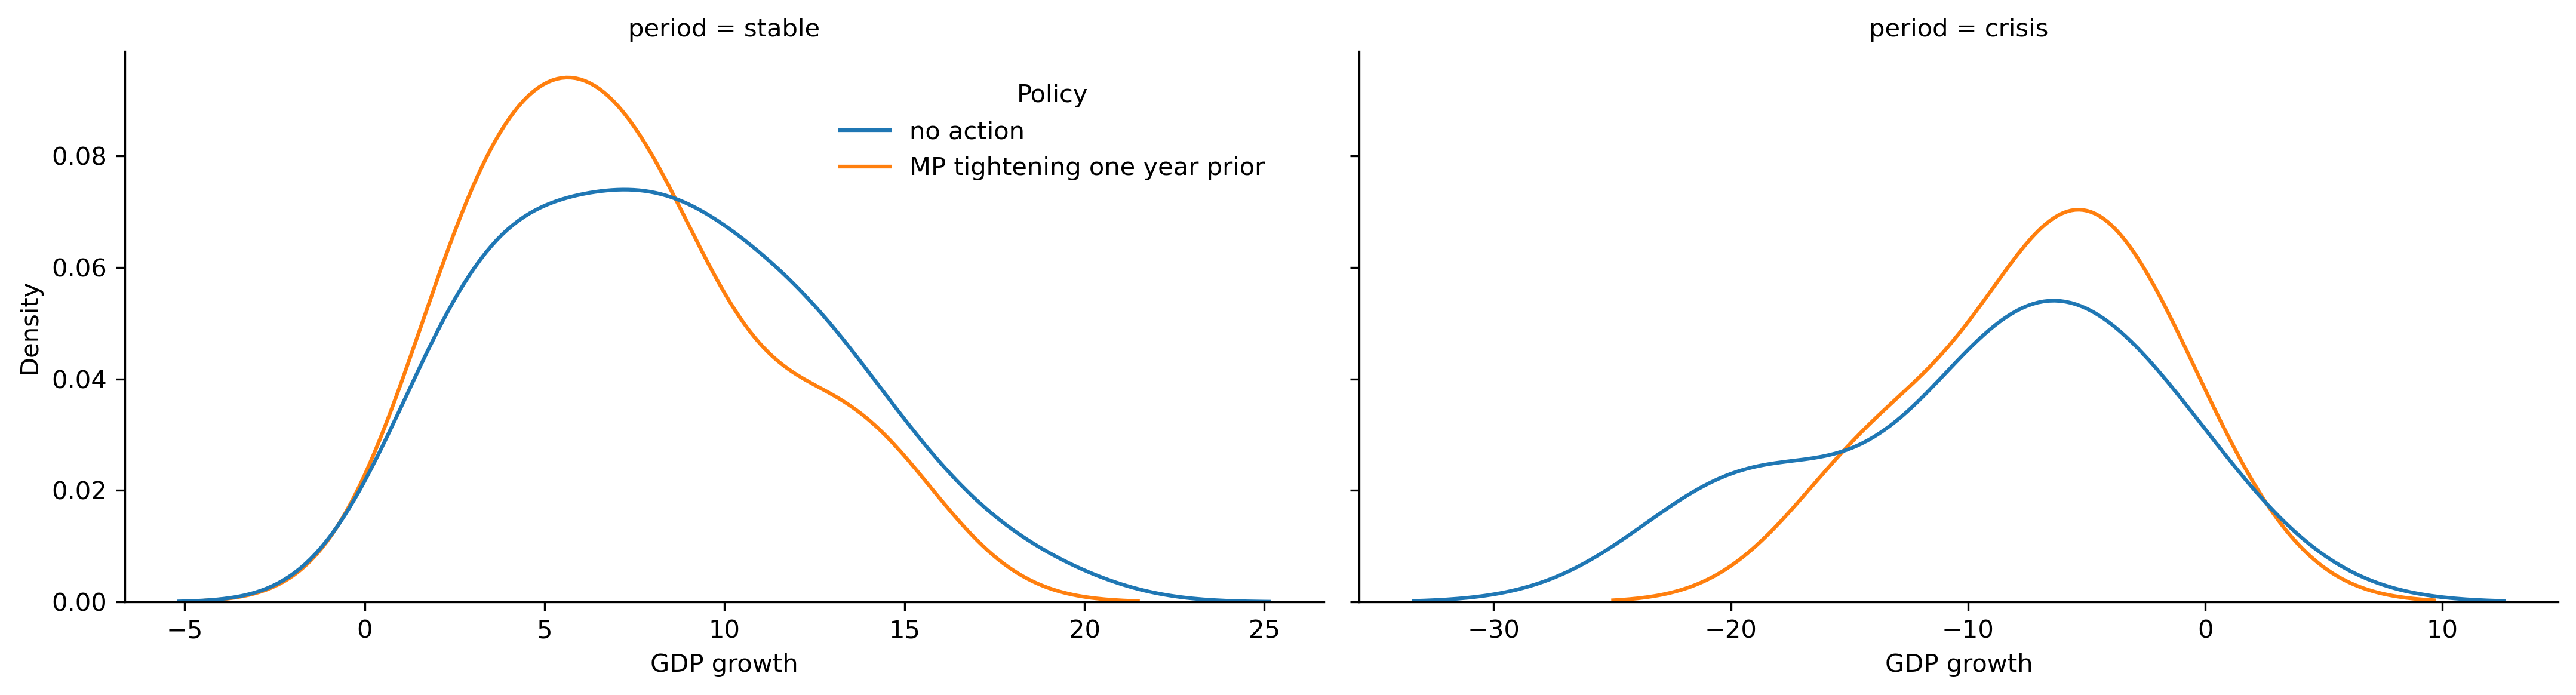
\includegraphics[width=1\textwidth, angle=0]{Figures/arm_MPI_tightening_gdp_dist.png}	
	\caption{GDP growth distribution of Armenia, one year after macroprudential policy tightening and during different economic phases.} 
	\label{fig:arm_MPI_tightening_gdp_dist}%
\end{figure*}
\begin{figure*}
	\centering 
	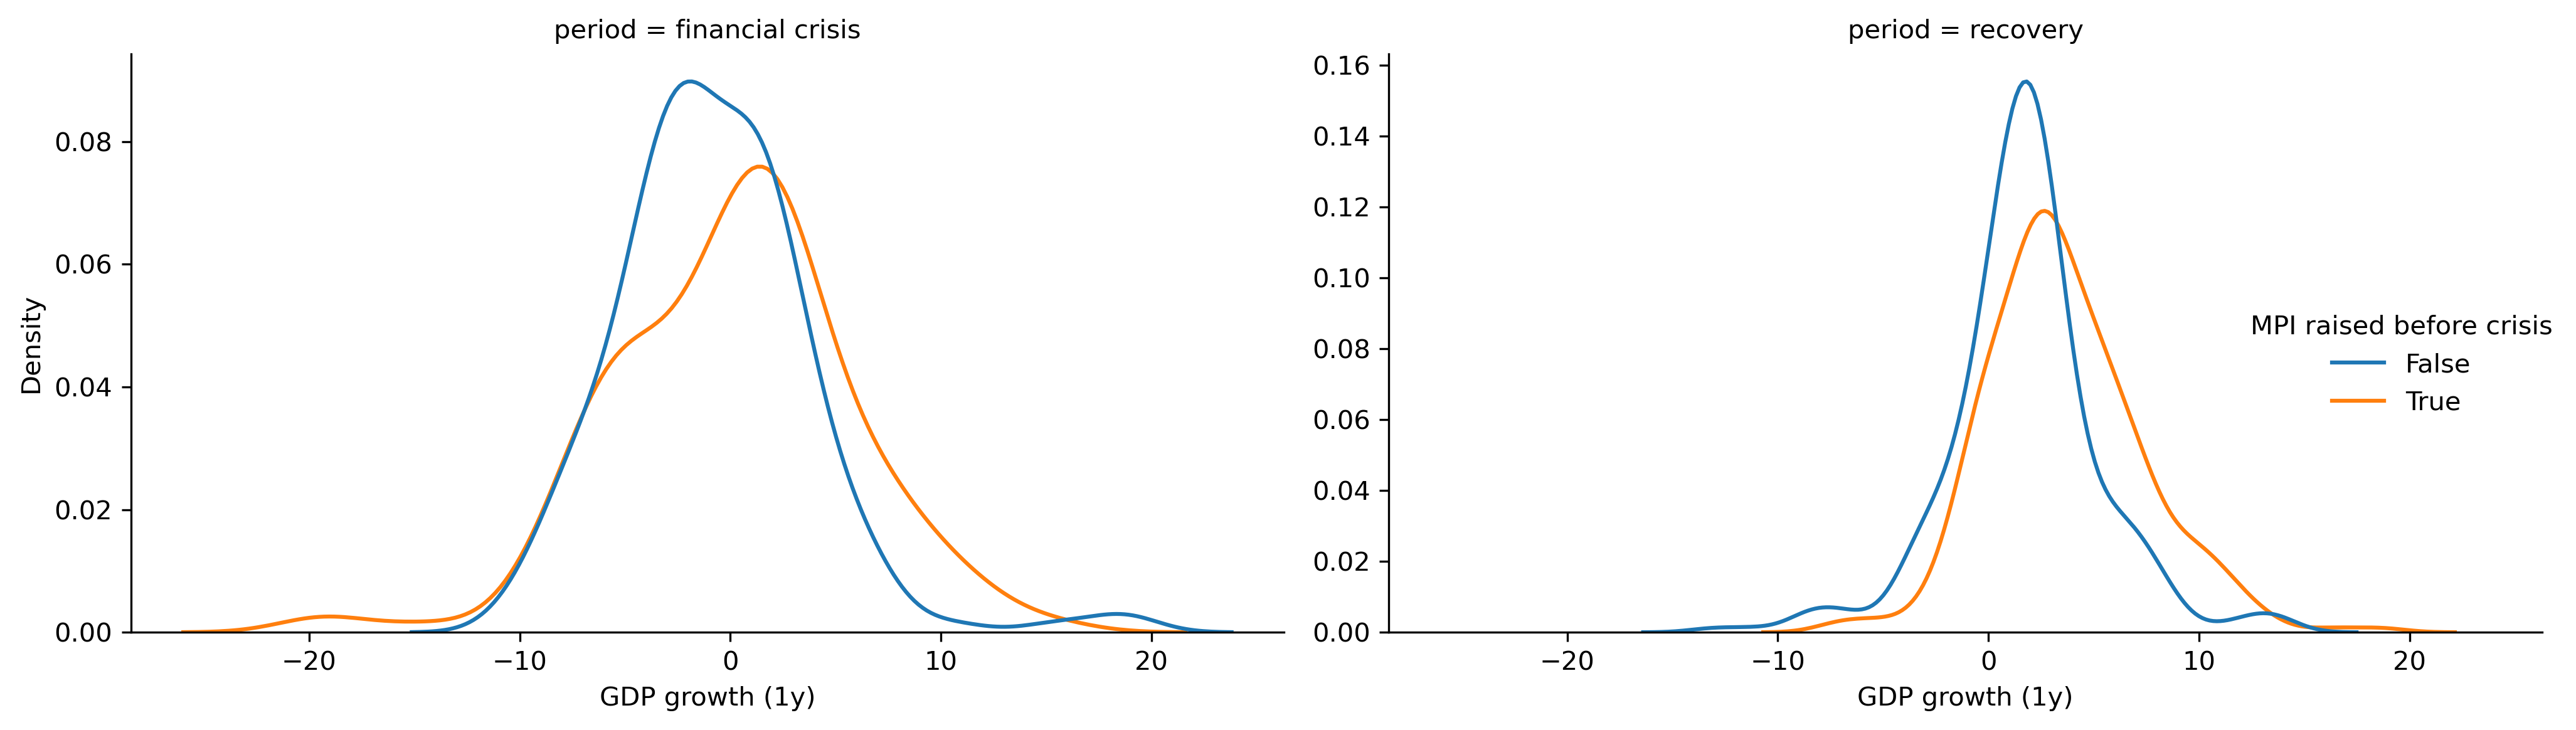
\includegraphics[width=1\textwidth, angle=0]{Figures/panel_MP_use_before_crisis.png}	
	\caption{GDP growth distribution of 41 countries that implemented macroprudential policy tightening one year before a major crisis.} 
	\label{fig:panel_MP_use_before_crisis}%
\end{figure*}
\begin{figure*}
	\centering 
	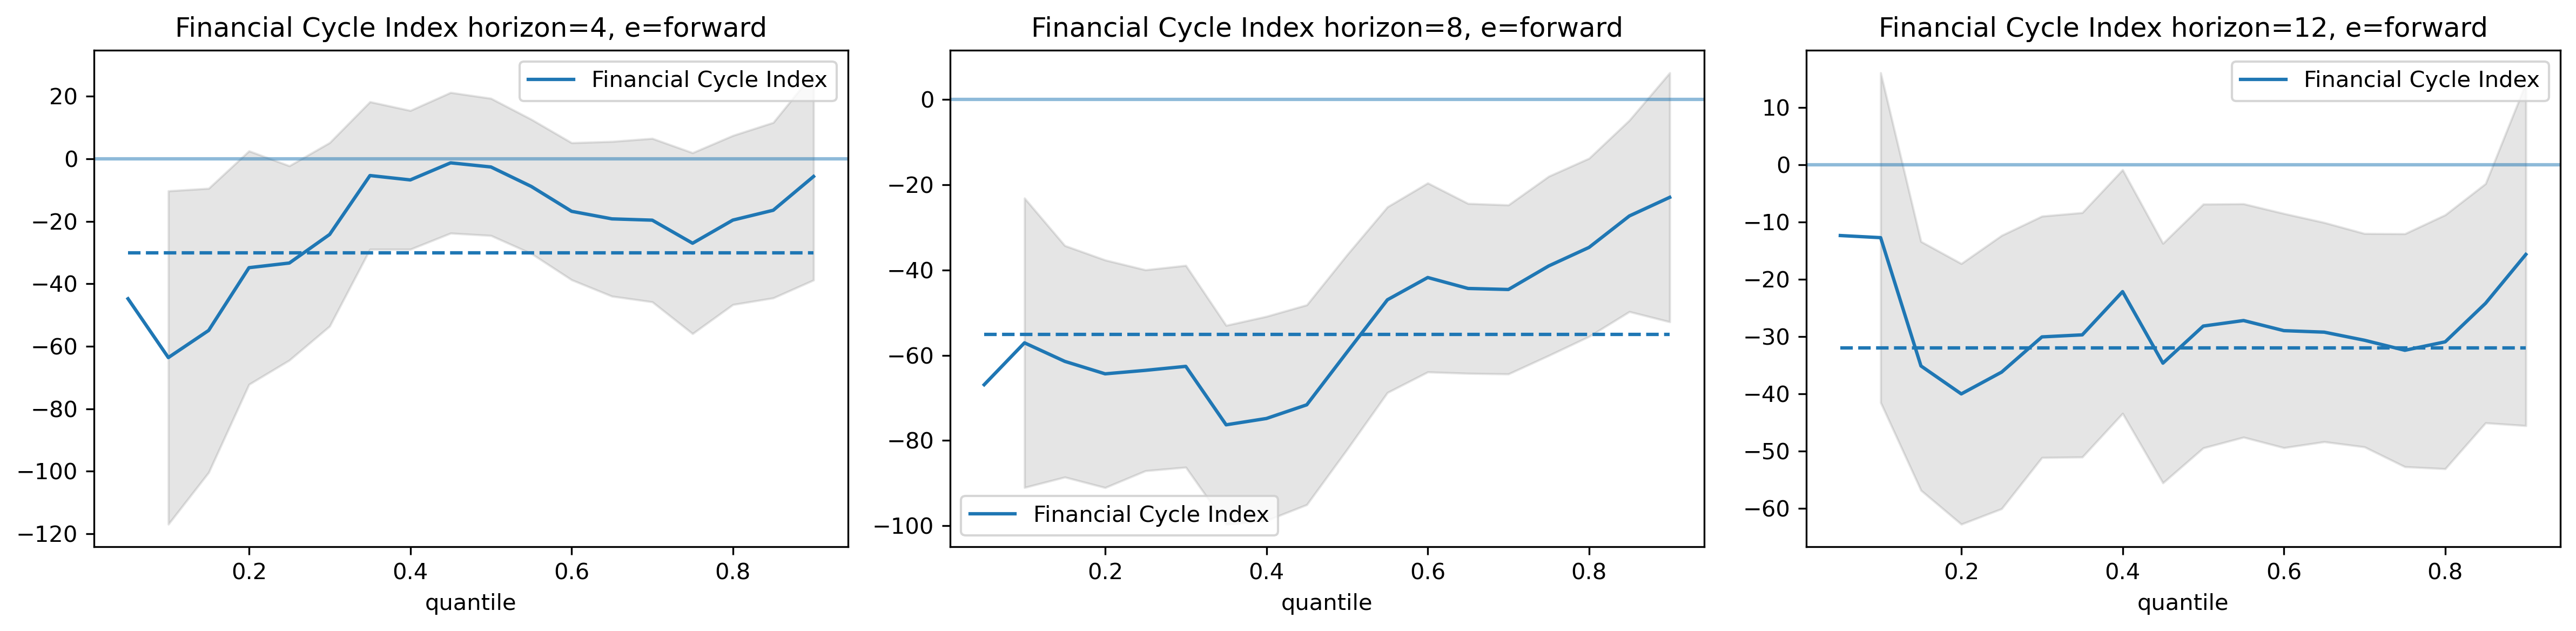
\includegraphics[width=1\textwidth, angle=0]{Figures/arm_FCyI_f_coeff_quantiles.png}	
	\caption{Local model Financial Cycle Index coefficients. Estimated quantile regression coefficients for horizons 4, 8, and 12. The grey-shaded areas represent the 95\% confidence intervals. The dashed horizontal line presents the OLS coefficient.}
	\label{fig:arm_FCyI_f_coeff_quantiles}%
\end{figure*}
\begin{figure*}
	\centering
	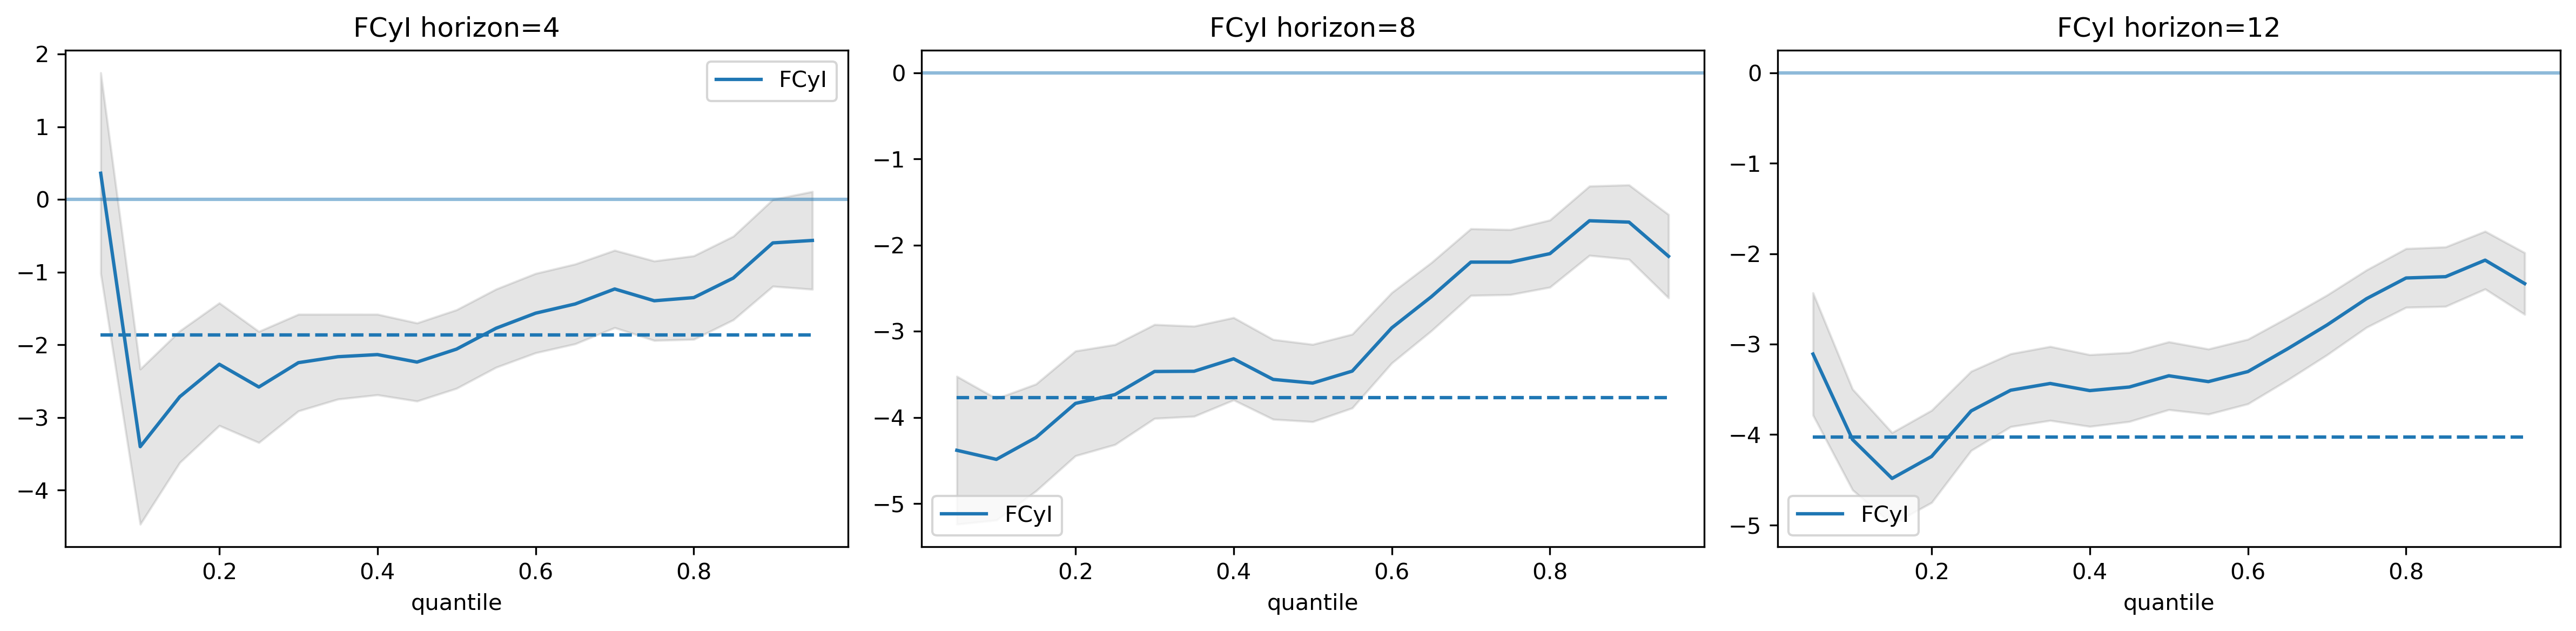
\includegraphics[width=1\textwidth, angle=0]{Figures/panel_FCyI_coeff_quantiles.png}	
	\caption{Panel model Financial Cycle Index coefficients.} 
	\label{fig:panel_FCyI_coeff_quantiles}%
\end{figure*}
\begin{figure*}
	\centering 
	
\includegraphics[width=1\textwidth, angle=0]{Figures/arm_FCI_f_coeff_quantiles.png}	
	\caption{Local model Financial Conditions Index coefficients. Estimated quantile regression coefficients for horizons 4, 8, and 12. The grey-shaded areas represent the 95\% confidence intervals. The dashed horizontal line presents the OLS coefficient.}
	\label{fig:arm_FCI_f_coeff_quantiles}%
\end{figure*}
\begin{figure*}
	\centering
	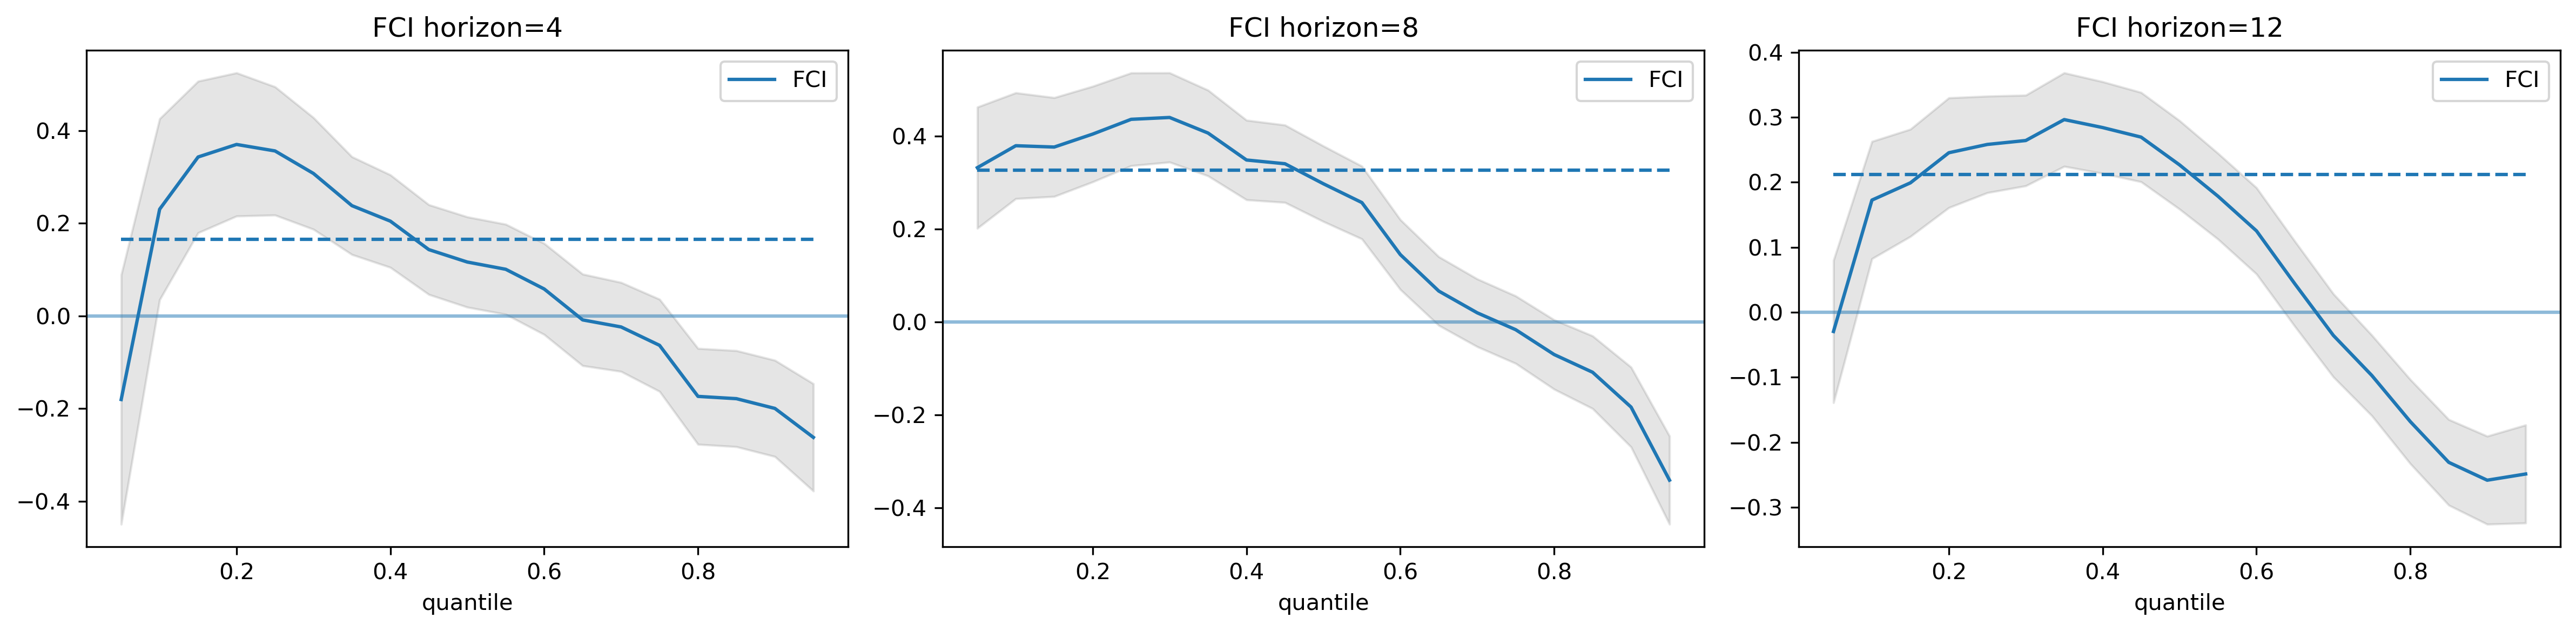
\includegraphics[width=1\textwidth, angle=0]{Figures/panel_FCI_coeff_quantiles.png}	
	\caption{Panel model Financial Conditions Index coefficients.} 
	\label{fig:panel_FCI_coeff_quantiles}%
\end{figure*}
\begin{figure*}
	\centering 
	
\includegraphics[width=1\textwidth, angle=0]{Figures/arm_MPI_f_coeff_quantiles.png}	
	\caption{Local model direct Macroprudential Policy Index coefficients. Estimated quantile regression coefficients for horizons 4, 8, and 12. The grey-shaded areas represent the 95\% confidence intervals. The dashed horizontal line presents the OLS coefficient.}
	\label{fig:arm_MPI_f_coeff_quantiles}%
\end{figure*}
\begin{figure*}
	\centering
	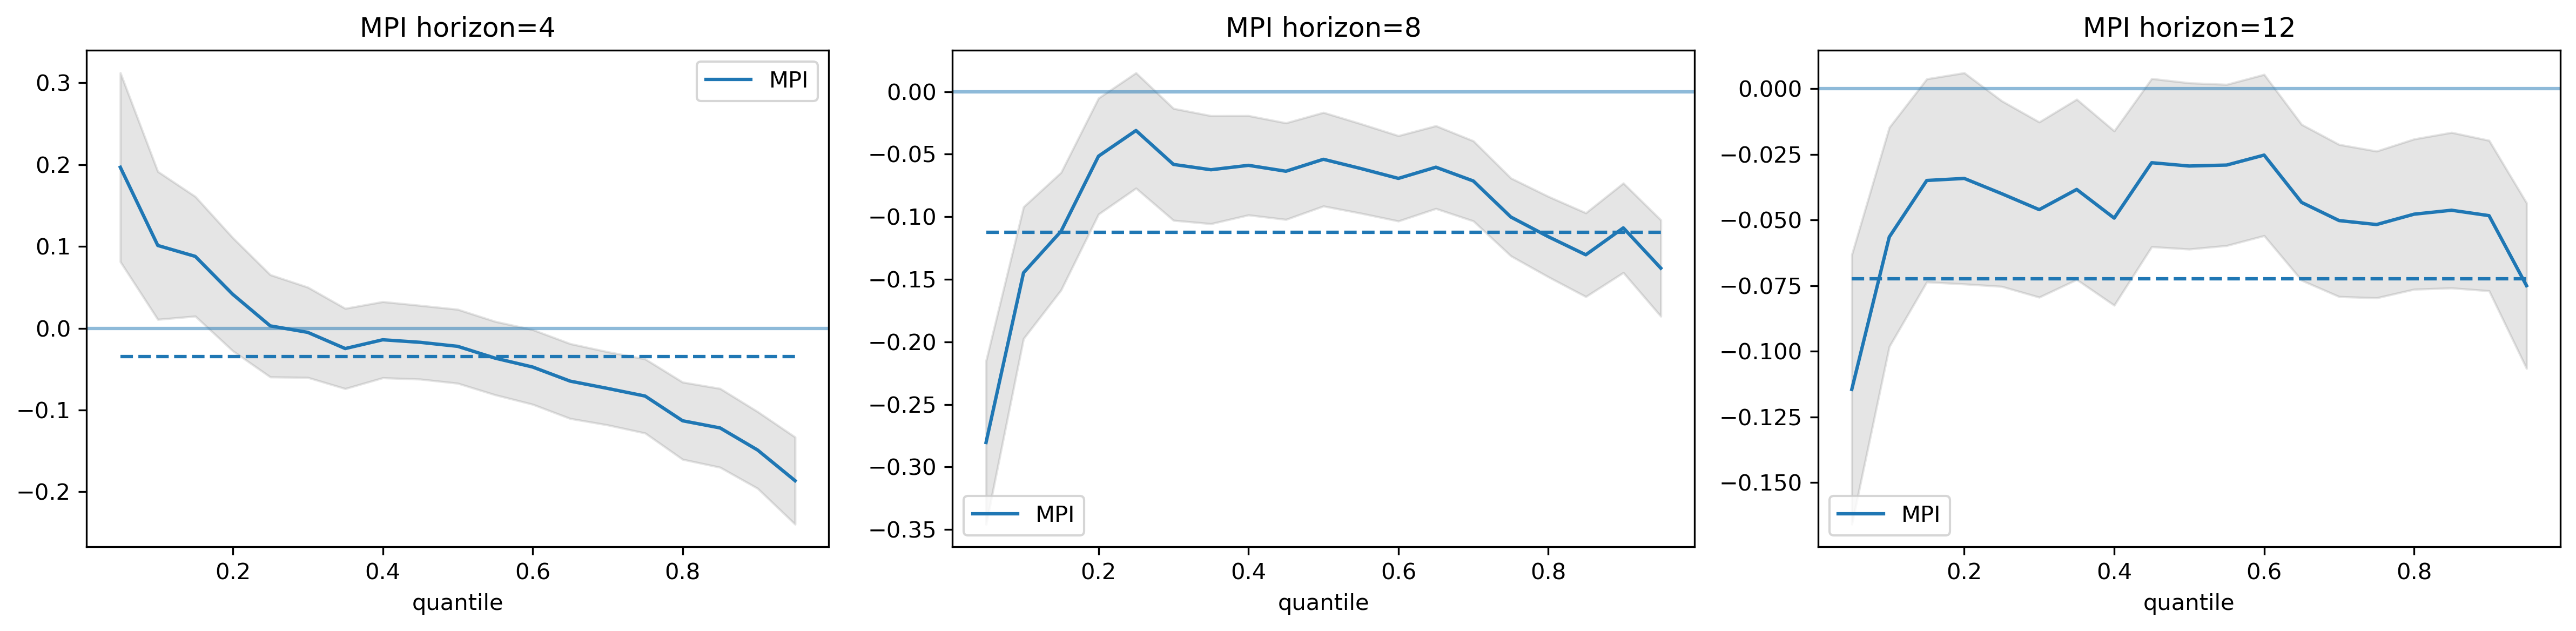
\includegraphics[width=1\textwidth, angle=0]{Figures/panel_MPI_coeff_quantiles.png}	
	\caption{Panel model direct Macroprudential Policy Index coefficients.} 
	\label{fig:panel_MPI_coeff_quantiles}%
\end{figure*}
\begin{figure*}
	\centering
	
\includegraphics[width=1\textwidth, angle=0]{Figures/arm_qr_gdp_dist.png}	
	\caption{Conditional GDP growth distribution of Armenia using skewed t-distribution fit for interpolation.}
	\label{fig:arm_qr_gdp_dist}%
\end{figure*}
\begin{figure*}
	\centering
	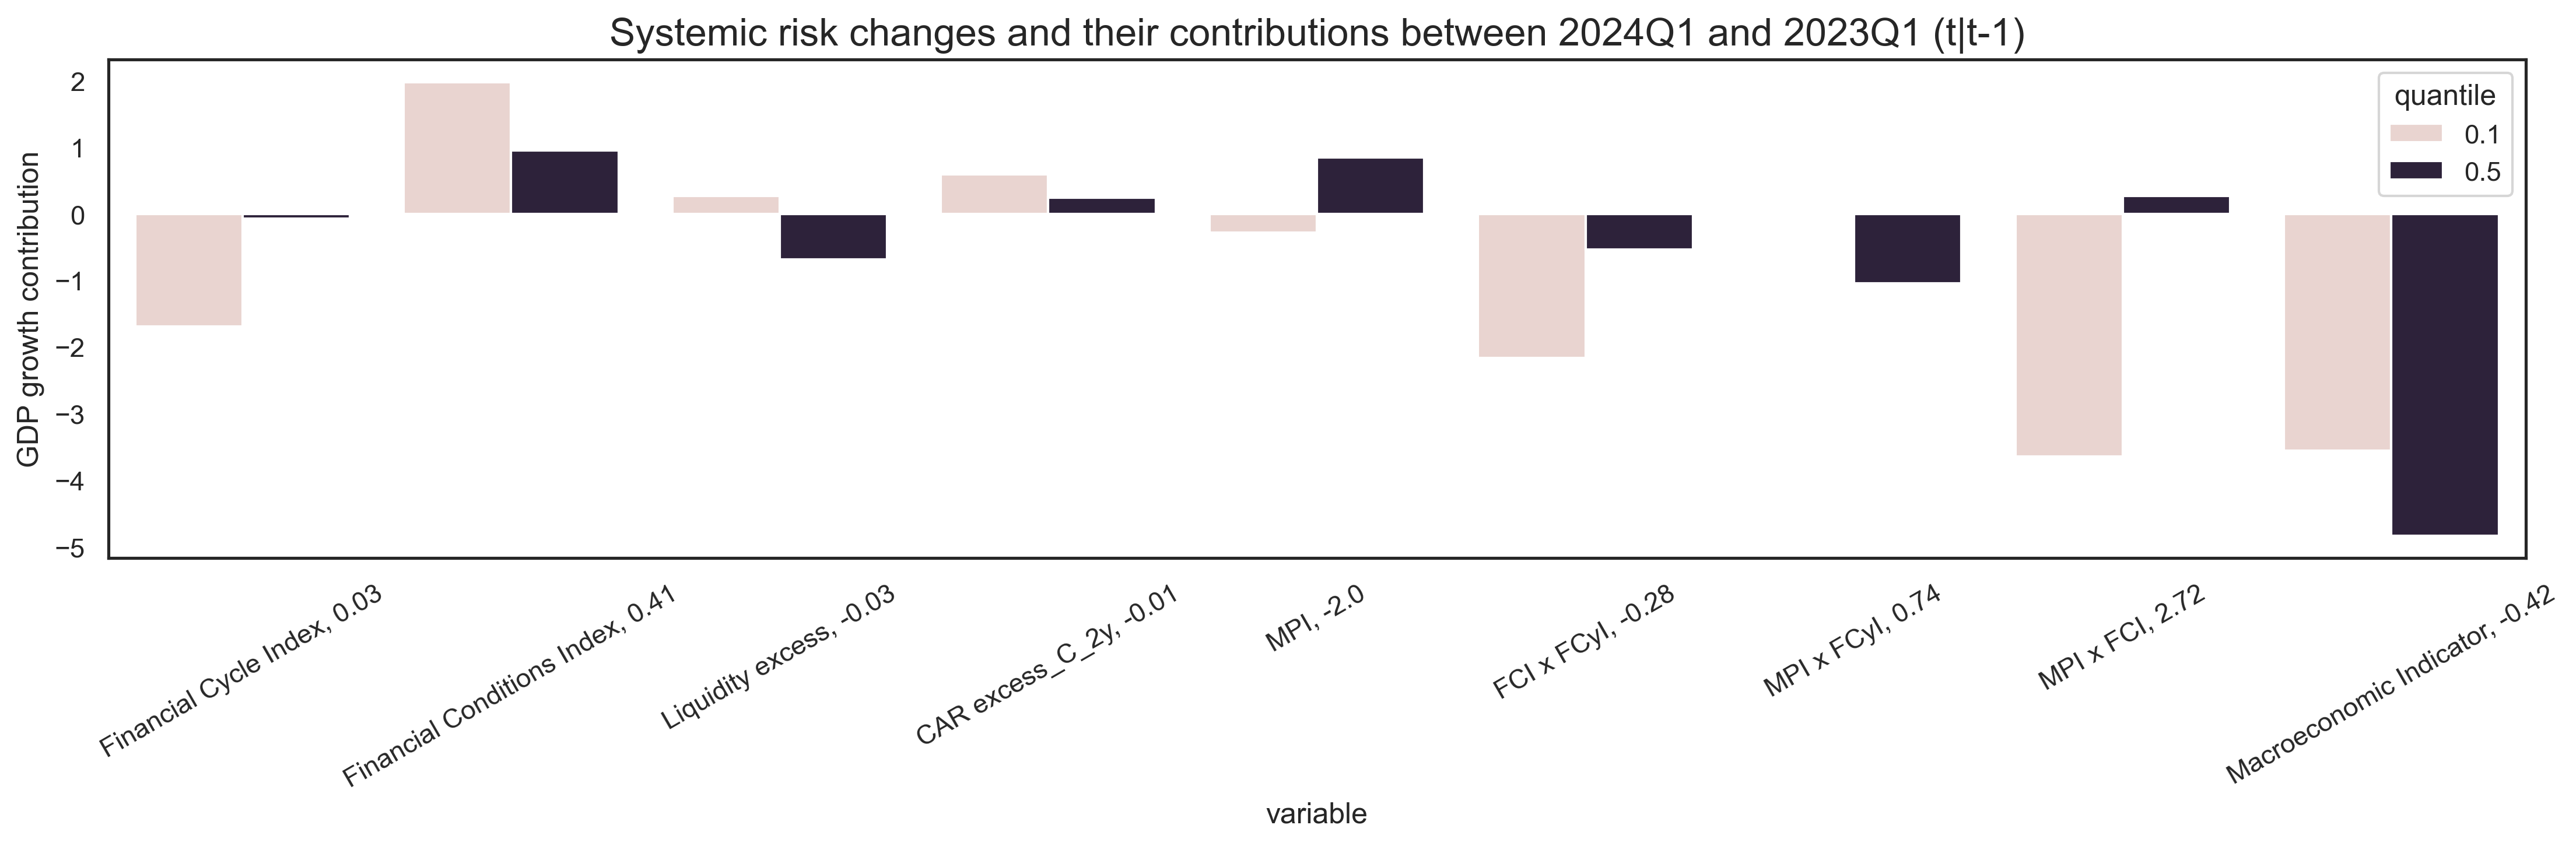
\includegraphics[width=1\textwidth, angle=0]{Figures/arm_dist_decomp_diff_2024Q1(t|t-1).png}	
	\caption{Changes in systemic risks between 2023Q1 and 2024Q1 and their impact on the GDP growth.}
	\label{fig:arm_dist_decomp_diff_2024Q1}%
\end{figure*}
\begin{figure*}
	\centering
	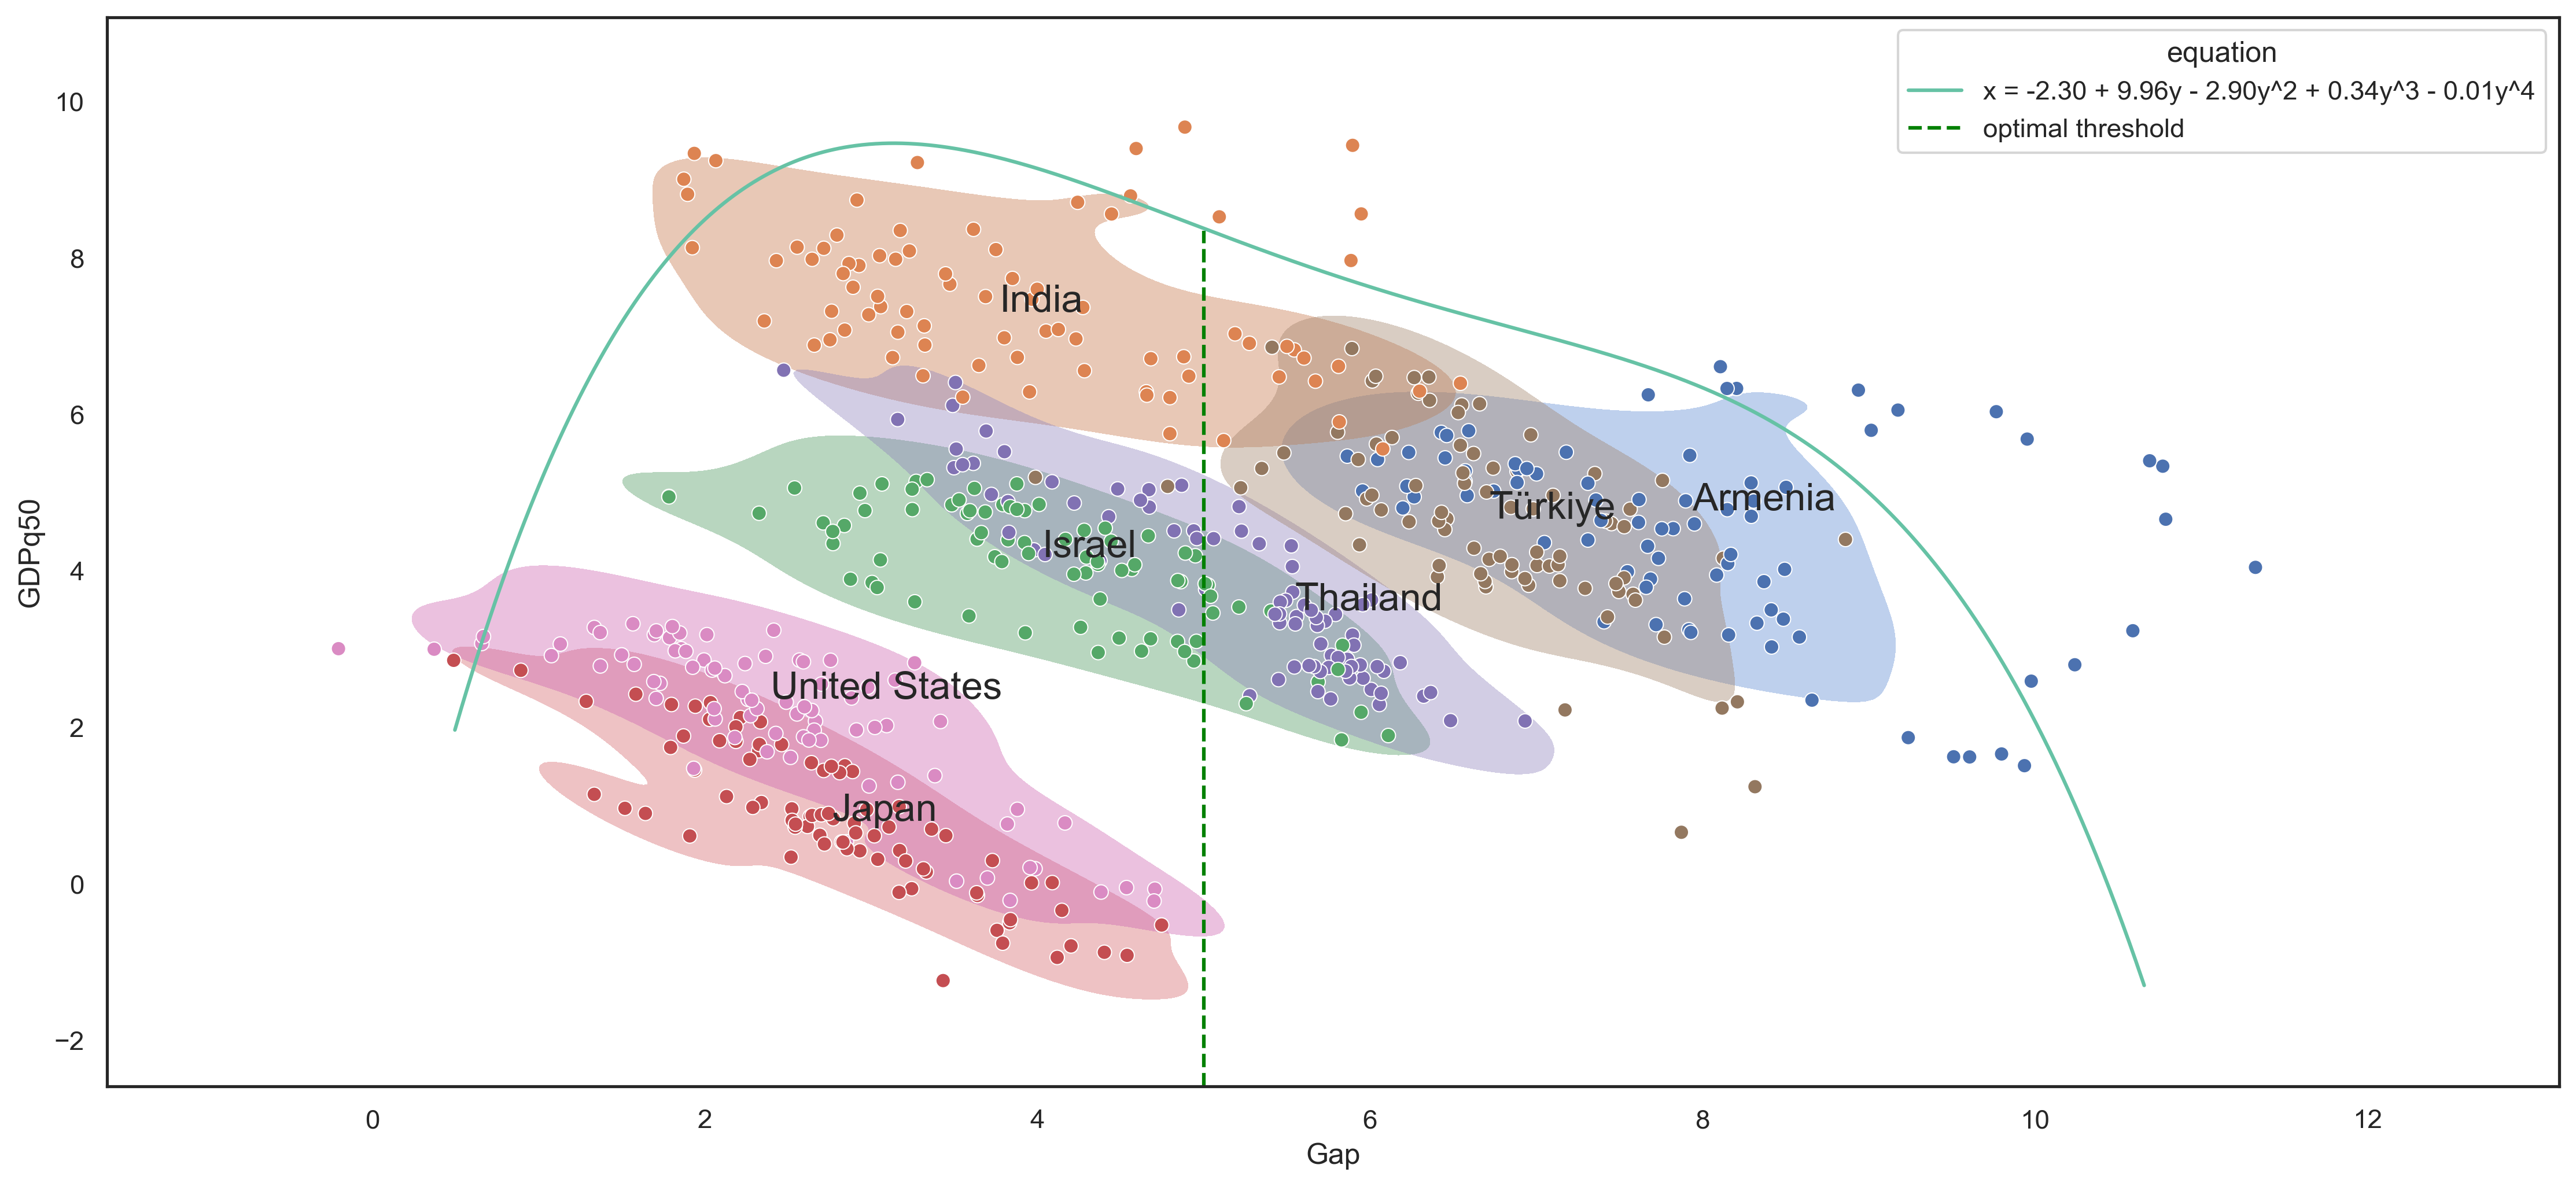
\includegraphics[width=1\textwidth, angle=0]{Figures/country_cases_that_shape_the_boundary.png}	
	\caption{Efficient frontier based on the median and distance-to-tail (Gap) estimates from the 41 countries. The green line represents the frontier and was estimated using a Local Outlier Factor (LOF) algorithm.}
	\label{fig:country_cases_that_shape_the_boundary}%
\end{figure*}